\section{競技性・観戦性を拡張したプログラミングゲームの開発}
本項では,プログラミング初学者の興味喚起を目的としたプログラミングゲームのプロトタイプについて紹介し,設計指針に基づくデザインの詳細や行った評価実験と見つかった課題,実験に関する考察について議論する.

\subsection{関連研究・関連システム}

\subsubsection{プログラミングを用いたエンタテインメントシステム}
プログラミングとエンタテインメントを掛け合わせたコンテンツはいくつか存在する.TopCoder\cite{topcoder}などの競技プログラミングやコードゴルフ\cite{codegolf},SECCON\cite{seccon}などのハッキングコンテストが有名であり,プログラマの間でも根強い人気がある.またプログラミングゲームとしてはRobocode\cite{robocode}が有名である.しかしこれらはある程度プログラミングに習熟したプログラマ向けのコンテンツであるため,数学やセキュリティ,コンピュータサイエンス等の知識を要するためプログラミング初学者が参加するにはハードルが高い.

\subsubsection{エンタテインメントを活用したプログラミング学習支援システム}
エンタテインメントの要素を盛り込むことでプログラミング学習を促進しようとした研究は多くある.Joshaらはプログラミングゲームを用いてプログラミング初学者の問題解決能力を向上させるためのシステムを作成している\cite{joshua}.また水口の研究ではプログラミングの講義における成績評価にロボットバトルシミュレーション型のプログラミングゲームを活用している\cite{minakuchi}.三谷らの研究ではキャラクタをプログラムで制御するプログラミングゲームでプログラミングスキルの向上を図っている\cite{mitani}.なお増谷らの開発したVLogic\cite{mashitani}ではVR空間上にブロックベースのプログラミングゲームを実装することで手足を使ってプログラミングを体験することができ,プログラミングに対する興味喚起を行っている.これらはプログラミングの習熟度が高くなくても使用できるが,従来のプログラミングゲーム同様静的なゲーム展開であり,プログラマ同士のリアルタイムな駆け引きやアドリブといった観戦を楽しむ設計は成されていない.

\subsection{設計指針}

提案システムの実装にあたり,初学者の興味関心を高めるために3つの設計指針を設けた.

\begin{enumerate}
	\item 観戦するにあたり,高度な専門知識を必要としない
	
	初学者が提案システムでの対戦を観戦するにあたり高度な専門知識を必要としてしまっては,利用の心理的ハードルを上げかねない.極力前提知識なしに理解し,楽しめるようにデザインする必要がある.
	
	\item 手間がかからない

	初学者にとってプログラミング学習をする際に環境構築や普段使用しない独自ソフトウェアのインストールはモチベーションを下げかねない.今回は提案システムをJavaScriptによって制御可能なWebアプリケーションとして実装し,初学者が実際にプログラミングを行わずとも見るだけで利用できるようにした.
	
	\item リアルタイムな駆け引き・アドリブを取り入れる

	従来のプログラミング教育コンテンツとは異なり,スポーツなどの観戦する競技で見られるようなリアルタイムな駆け引き・アドリブの要素を提案システムに組み込むことで観戦して楽しめるようなデザインをする.
\end{enumerate}

\subsection{提案システム}

本研究で提案するシステムでは,プログラミング初学者の興味喚起をするためにいくつかの工夫を施した.今回実装したシステムは,プログラマ同士がリアルタイムにプログラミングを行うことでキャラクタを制御し,対戦するという対人形式のプログラミングゲームである.この対戦の様子を初学者に観戦させることで,初学者のプログラミングに対する興味を高める.プログラミングゲームとして実装した理由としては,キャラクタがプログラムによって動作するというゲームの視覚的な出力が,初学者にとってプログラムの出力を理解する助けになると考えたためである.ゲームジャンルとしては,シューティングゲームの体裁をとった.これはシューティングゲームが「敵の攻撃を避けて,敵を攻撃する」というプリミティブなゲームシステムであり,見ていて展開を理解しやすいと考えたためである.またゲームUIはLivecodeLabやHydraなどのビジュアルライブコーディング環境を踏襲し,ゲーム画面上にエディタを重畳することで,プログラムとその出力の双方を同時に見ることが可能なように設計した.またゲームは以下の3つのフェイズに分かれている.

\subsubsection{自機プログラミングフェイズ}
対戦が開始するとこのフェイズに移行する.ここでは予めエディタにプレイヤが操作するキャラクタのコンストラクタが記述されており,プレイヤはパラメータを書き換えることができる.具体的なパラメータにはappearance,life,clock,powerがある.appearanceはキャラクタの外見であり,文字列を指定できるため,絵文字などを使ってプレイヤの好きな見た目を選ぶことが可能である.lifeはキャラクタの体力であり,いわゆるHP(ヒットポイント)を表している.非負の整数を指定でき,この値が0以下になるとプレイヤはゲームに敗北する.clockはキャラクタが行動できる回数の多さを表しており,非負の整数を指定できる.プレイヤは後述する行動プログラミングフェイズにおいて自分のキャラクタを制御するプログラムを記述し対戦するが,その際に記述したプログラムは10秒間ループして実行される.このループのインターバルを決めるのがclockであり,値が大きいほどインターバルは短くなる.powerはキャラクタの攻撃力を表しており,これも非負の整数を指定できる.この値が大きいほど,自分が操作するキャラクタの攻撃が相手キャラクタに命中した際に削るlifeの値が大きくなる.双方のプレイヤが各パラメータを記述し終わると次の行動プログラミングフェイズに移行する.このフェイズの様子を図\ref{characterProgramming}に示す.

\begin{figure}[!h]
  \begin{center}
    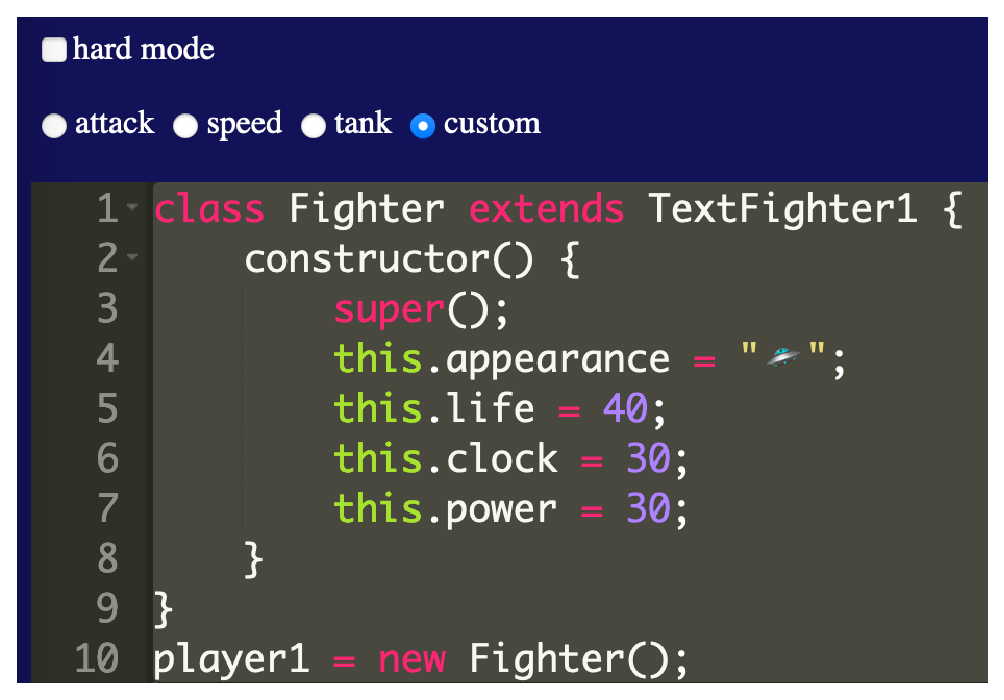
\includegraphics[width=1.0\linewidth]{image/characterProgramming.eps}
  \end{center}
    \vspace{-8mm} 
  \caption{自機プログラミングフェイズの様子}
  \label{characterProgramming}
\end{figure}

\subsubsection{行動プログラミングフェイズ}
このフェイズに進むと,自機プログラミングフェイズで記述したコンストラクタを元に各プレイヤが操作するキャラクタのインスタンスが作成され,ゲーム画面が表示される.各プレイヤはプログラムをエディタに記述し,作成したキャラクタを操作する.プレイヤは条件分岐や繰り返しなど従来のJavaScriptの文法の他に独自に用意されたプロトタイプメソッドを使うことができる.用意したメソッドにはキャラクタを移動するメソッド(moveUp(), moveDown(),randomMove())とキャラクタが攻撃を行うメソッド(shot())などがある.またプログラム内で各キャラクタのパラメータを参照することもできる.両プレイヤがプログラムを記述し終わると次のゲームフェイズに移行する.なおこのフェイズでは相手プレイヤがどのようなプログラムを記述しているかは見ることができない.このフェイズの様子を図\ref{actionProgramming}に示す.

\begin{figure}[!h]
  \begin{center}
    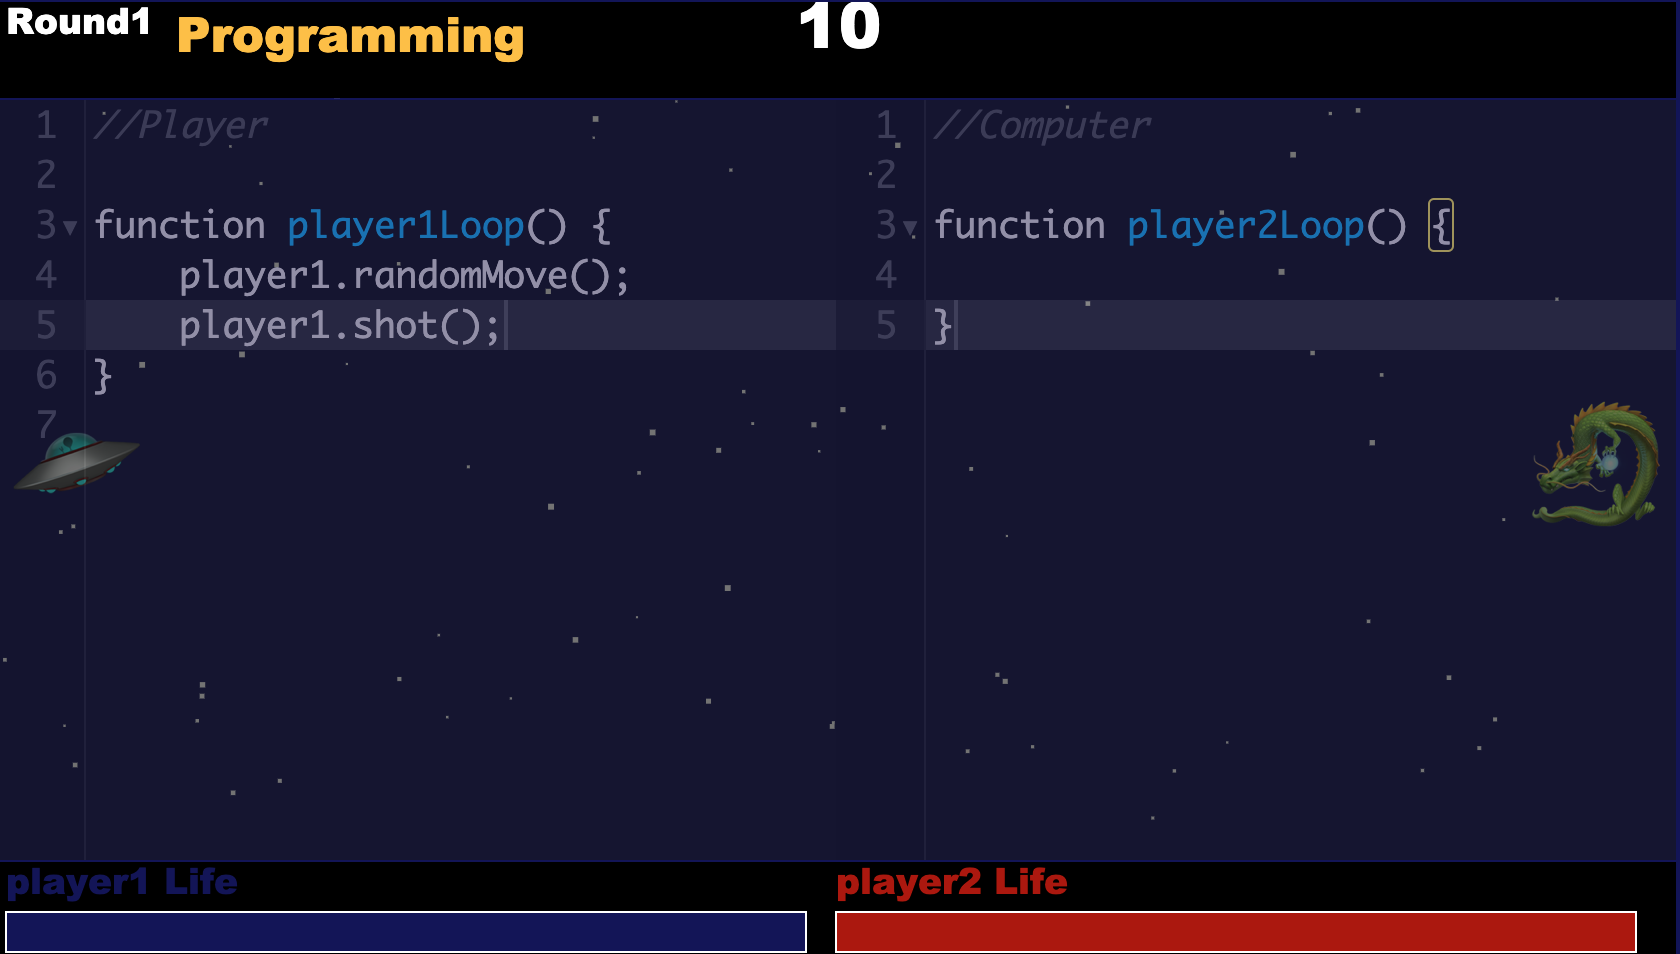
\includegraphics[width=1.0\linewidth]{image/actionProgramming.eps}
  \end{center}
    \vspace{-8mm} 
  \caption{行動プログラミングフェイズの様子}
  \label{actionProgramming}
\end{figure}

\subsubsection{ゲームフェイズ}
このフェイズでは行動プログラミングフェイズで記述したプログラムが10秒間ループして実行され,ゲームが進行する.この段階で両プレイヤは相手プレイヤが記述したプログラムを閲覧することができる.このフェイズにおいて相手キャラクタを攻撃し,lifeの値を0いかにしたプレイヤの勝利となる.勝敗が決まらない場合はプログラム終了時の各パラメータを引き継いだまま行動プログラミングフェイズに戻り,再度プログラミングしゲームフェイズに移行するという過程を勝敗が決まるまで繰り返す.このフェイズの様子を図\ref{game}に示す.

\begin{figure}[!h]
  \begin{center}
    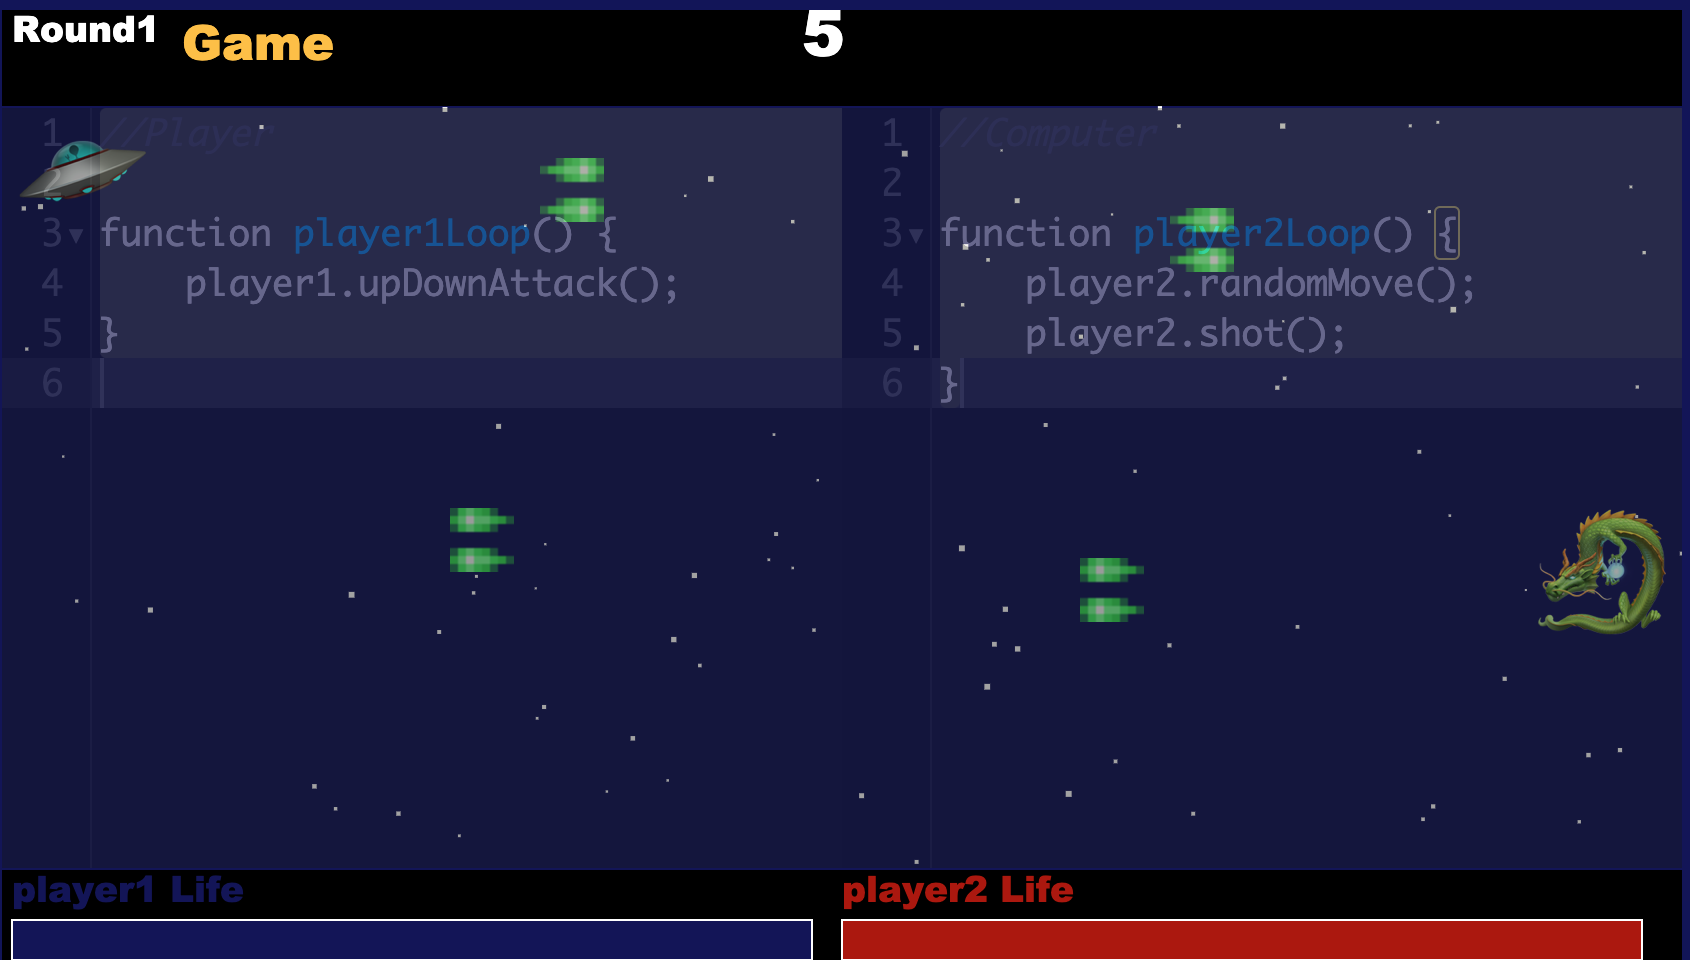
\includegraphics[width=1.0\linewidth]{image/game.eps}
  \end{center}
    \vspace{-8mm} 
  \caption{ゲームフェイズの様子}
  \label{game}
\end{figure}

\subsection{評価実験}
提案システムの使用・観戦に関する感想や影響,用法を調査するために評価実験を実施した.システムをプレイするプログラマと観戦するプログラミング初学者を集め,システムでの対戦と観戦を実施し,アンケート調査と実際に対戦で使用されたプログラムのログを分析することでシステムを評価した.

\subsubsection{実験参加者}
実際にゲームをプレイするプログラマとしては,プログラミング(主にオブジェクト指向言語)の経験が3年以上ある大学院生2名(男性)に声をかけた.2名とも日常的にアクションやシューティング等のジャンルのゲームをプレイするため,システムをプレイする際にゲームに不慣れなためハンデが生まれることはないと思われる.また両者とも3年以上JavaScriptを使用した経験がある.
またプレイを観戦するプログラミング初学者は,国際人間科学部にて開講されていた講義「プログラミング基礎演習1」の受講者をとした.受講者のうち,実験に参加した者は77名であり,うち37名が男性,40名が女性であった.またこの講義ではJavaScriptにおける変数,条件分岐,繰り返しなどの基礎的な文法を教えており,実験参加者は実験を行う時点でこれらを学習済であった.なお,うち23名は授業以前にプログラミングを学習した経験があったが,ソフトウェア開発を行ったことのある者はいなかった.
またプログラマ含む実験参加者の全員が,競技プログラミングやプログラミングゲームなどのプログラミングを題材としたエンタテインメントを使用した経験がなかった.

\subsubsection{実験内容}

初めにプログラマ2人に簡単な事前アンケートを行った後,提案システムにある程度慣れ,用法を理解してもらう必要があるため,システムの練習をするための期間を設けた.システムの使用方法,ゲームシステム,独自に用意したメソッドなどについて説明した後,11/13から11/19の1週間システムを自由に使用させた.また,ただシステムを使用させただけではゲームに対する理解度が上がらない可能性があるため,期間中に2つのタスクをこなさせた.1つは1人以上とシステムを使った対人戦を行うことであり,もう1つは相手がランダムな戦略を実行してくる対CPU戦において,勝率が高いと考えられるプログラムを作成することである.なお期間中はシステムに関する意見・疑問を逐次報告させ,システム使用における問題を改善した.
練習期間が終わった翌日に,プログラマ同士の対戦を行った.対戦はシステムに関するプログラマ同士のコミュニケーション等の所作を観察するため,感染症対策を徹底した環境で対面にて行った.両者の対戦時の画面を録画し,対戦後にシステムに関する事後アンケートを行った.なお練習期間中・対戦中にプログラマが記述した全てのコードのログを収集した.
そして「プログラミング基礎演習1」の最終講義で受講者に事前アンケートを行った後,初学者が観戦しやすいように対戦動画を編集したものをzoomを介して閲覧させた.またその後にシステムに関する事後アンケートを行った.

\subsubsection{実験結果}

\begin{enumerate}
	\item アンケート結果

	\item コードログ分析結果
\end{enumerate}

\subsubsection{考察}
評価実験に関する考察について述べる.プログラマ同士の対戦においては,行動プログラミングフェイズで設定したappearanceについて「かわいい」などとコメントしていた.また対戦後にお互いのプログラムの内容や今までのプログラミング経験に関するコミュニケーションをとっており,システムを使用することでプログラマ同士のコミュニケーションを促進できていたと考えられる.
初学者の対戦の観戦においては,ライブでプログラマ同士が対戦している状況を用意することが困難であったため今回は動画を閲覧するという状況を用意したが,動画を見ただけでは実際に人が対戦しているという感覚が希薄であり,「プログラマがプログラミングしている」場面を見せるためには更なる工夫が必要であると感じた.
また今回の評価実験において,システムに対する肯定的な評価が得られたものの,どのような要素が初学者のプログラミングに対する興味に影響を与えていたのか,特に提案システムにおいて独特な要素であるリアルタイムな駆け引き・アドリブを誘発する要素の影響について調査する必要があると考えられる.

\subsection{課題}





